 %%	SECCION documentclass																									 %%	
%%---------------------------------------------------------------------------%%
\documentclass[a4paper]{report}

%%---------------------------------------------------------------------------%%
%%	SECCION usepackage																											 %%	
%%---------------------------------------------------------------------------%%
\usepackage{amsmath, amsthm}
\usepackage[spanish,activeacute]{babel}
\usepackage{caratula}
\usepackage{a4wide}
\usepackage{hyperref}
\usepackage{fancyhdr}
\usepackage{graphicx} % Para el logo magico!
\usepackage{amssymb}
\usepackage{amsmath}
\usepackage[latin1]{inputenc}
%\usepackage [T1]{fontenc}
\usepackage[dvipsnames,usenames]{color}
\usepackage{amsfonts}
\usepackage{ulem}
%\usepackage{highlight}
\usepackage{fancybox}
%\usepackage{marvosym}
\usepackage{color}
\usepackage{lastpage}

%%---------------------------------------------------------------------------%%
%%	SECCION opciones																												 %%	
%%---------------------------------------------------------------------------%%
\parskip    = 11 pt
\headheight	= 13.1pt
\pagestyle	{fancy}
\definecolor{orange}{rgb}{1,0.5,0}

\addtolength{\headwidth}{1.0in}

\addtolength{\oddsidemargin}{-0.5in}
\addtolength{\textwidth}{1.0in}
\addtolength{\topmargin}{-0.5in}
\addtolength{\textheight}{0.7in}

%%---------------------------------------------------------------------------%%
%%	SECCION document	 %%	
%%---------------------------------------------------------------------------%%
\begin{document}
\renewcommand{\chaptername}{Parte }

%%---- Caratula -------------------------------------------------------------%%
\materia{Ingenier�a del Software II (2do cuatrimestre de 2009)}
\titulo{Trabajo Pr�ctico I - Segunda Entrega}

\integrante{Castillo, Gonzalo}{164/06}{gonzalocastillo\_086@hotmail.com}
\integrante{Elizalde, Victoria}{452/06}{kivielizalde@gmail.com}
\integrante{Gonzalez, Sergio}{481/06}{gonzalezsergio2003@yahoo.com.ar}
\integrante{Page Saal, Mart�n}{315/06}{martinpage2001@yahoo.com.ar}
\resumen{
En el siguiente documento, se arribar� un sprint de Scrum intentando tambi�n de algun modo, adaptar la arquitectura a los nuevos requerimientos solicitados, para poder seguir cumpliendo los objetivos del proyecto.}

% TOC, usa estilos locos
\maketitle
\pagestyle{empty}
{
\fancypagestyle{plain}
    {
    \fancyhead{}
    \fancyfoot{}
    \renewcommand{\headrulewidth}{0.0pt}
    } % clear header and footer of plain page because of ToC
\tableofcontents
}

\newpage
% arreglos los estilos para el resto del documento, y
% reseteo los numeros de pagina para que queden bien
\pagenumbering{arabic}
\fancypagestyle{plain} {
    \fancyhead[LO]{Castillo, Elizalde, Gonzalez, Page Saal}
    \fancyhead[C]{}
    \fancyhead[RO]{P\'agina \thepage\ de \pageref{LastPage}}
    \fancyfoot{}
    \renewcommand{\headrulewidth}{0.4pt}
}
\pagestyle{plain}

\newpage
\chapter{Introducci�n}

\section{Notaci�n}

Agregaremos unos pocos t�rminos nuevos que se utilizaran a lo largo de este documento. 

\begin{itemize}
	\item ECP : Estaci�n Central Provincial
	\item SMP : Sistema de Monitoreo Provincial
\end{itemize}

\section{Introducci�n}

En esta segunda parte del proyecto, nos encontramos con una serie de requerimientos, que son nuevos y que se agregan a los que se ten�an en la primera parte. Adem�s de esto, se contin�a con el crecimiento del proyecto con una metodolog�a diferente a la que se ven�a utilizando, esta metodolog�a es scrum, y como funciona de manera iterativa e incremental, adem�s de funcionar diferente a UP, se tuvo que adaptar a esta nueva forma de pensar el problema, e ir avanzando en el proyecto.

As� es de esta forma, en lo que sigue de este informe, se ver�n todas estas nuevas caracter�sticas, expuestas en las diferentes secciones. Para adaptarnos a los nuevos requerimientos, en la fase de planificaci�n, identificamos las funcionalidades mas importantes que tiene que tener el sistema y las agrupamos en epics. Vale aclarar que estas nuevas funcionalidades impulsaron un cambio en la arquitectura que se expuso anteriormente en la primera entrega, pero estos cambios no fueron tan graves. Tambi�n se realiz� el product backlog, y el sprint backlog con los user stories que se tienen que incluir seg�n lo pedido, con sus respectivas estimaciones, teniendo en cuenta la duraci�n del sprint que es de 2 semanas. Las etapas que se pusieron en pr�ctica son las siguientes:

\begin{itemize}

\item Planeamiento: En esta etapa se identificaron los nuevos requerimientos que se agregaron al sistema y se pusieron los epics relacionados. Tambi�n se realiz� el sprint backlog con los user stories que se corresponden con los nuevos requerimientos y los epics. Estos user stories son los que se espera que tenga el sistema al final cuando se termine.

\item Realizaci�n del sprint backlog: Aqui se tomaron los user stories que deben entrar para esta entrega, cada uno de estos fue estimado, estimando primeramente las tareas en las que fueron descompuestos cada uno, llegando a un consenso y luego en base a esto se asignaron esfuerzos a cada uno.

\item Casos de aceptaci�n: Algo que no estaba pedido en el enunciado expl�citamente, pero que nos pareci� correcto poner para agregar mas informaci�n en relaci�n a la finalizaci�n de cada user storie.


\end{itemize}

Luego de esto, se explican con detalle los cambios realizados a la arquitectura, donde surge el concepto de estaci�n central provincial (ECP), estaciones que estar�n en cada provincia, teniendo como funci�n principal, el procesamiento de los datos que le brindan las TRs de la zona, adem�s de la colaboraci�n con otras estaciones centrales, brind�ndoles informaci�n de su �rea como ser informaci�n de TRs, como resultados de los modelos.

Adem�s de lo mencionado anteriormente, se tuvo que realizar el dise�o de la secci�n relacionada con la ejecuci�n de los modelos matem�ticos, que en este caso, tiene que realizarse de forma distribuida. Para esto se hizo un dise�o, donde se detalla el funcionamiento que tendr� esta funcionalidad en el sistema. Dicho dise�o, es un diagrama de clases, y para describir el funcionamiento de la colaboraci�n de los objetos, se realiz� un diagrama de objetos y diversos diagramas de secuencia (de colaboraci�n). De esta forma queda bien explicado el funcionamiento de la ejecuci�n en forma distribuida de las reglas de un modelo, como se pide en el enunciado del trabajo.

Por �ltimo, se realiz� una comparaci�n entre el proceso de scrum y el proceso UP de desarrollo de sofware, donde incluimos opiniones al respecto.
\clearpage

\newpage
\chapter{Objetivo del sprint}

La caracter�stica principal de �ste sprint es la aparici�n de nuevos requerimientos funcionales.  Esto hace que se tenga que pensar como se adec�a la arquitectura a dichos requerimientos y en caso de ser necesario, c�mo deber�a modificarse para contemplar los mismos, teniendo en cuenta que funcione todo lo hecho hasta el momento. Entonces, b�sicamente el objetivo del sprint es adaptar la arquitectura pensada en la primera entrega del trabajo pr�ctico a los nuevos requerimientos, y llevar a cabo la nueva planificaci�n utilizando scrum. Una vez hecho esto debemos seleccionar la lista de stories que llevaremos a cabo en el sprint, estimarlos (utilizando valores relativos, que luego se traducir�n a esfuerzo) y comenzar con su implementaci�n para lograr un adecuado product increment que sea aceptado por el usuario.

Ser� necesario pensar c�mo van a impactar los nuevos requerimientos en la arquitectura ya dise�ada y como realizar un adecuado trade off para seguir garantizando el cumplimiento de los antiguos requerimientos y la satisfacci�n de los nuevos.

Tambi�n se espera tener los primeros stories realizados, que se corresponden con los que se indican en el enunciado del trabajo, resolviendo los problemas que surjan en el trayecto del mismo. Este avance se ver� reflejado en el Sprint Burndown Chart final, y se podr� observar como fue evolucionando el sprint durante las 2 semanas que dura.

Se espera fijar ademas las ideas cuando se tengan dudas acerca del proyecto su avance y su desarrollo cuando tengamos las stand-up meetings correspondientes, corroborando el seguimiento del proyecto.
\clearpage


\newpage
\chapter{Planificaci�n}	

En �ste cap�tulo se llevar� a cabo la planificaci�n de proyecto en general. Se denotar�n epics, para dar una vision global de las funcionalidades a implementar, los User Stories correspondientes asociados a los requerimientos solicitados, y finalmente el Sprint Backlog, con el subconjunto de los requerimientos a implementar en el sprint. Es importante comunicar que seguiremos cada uno de los puntos del enunciado, es decir la lista de User Stories, aquellos que entren en el sprint junto a sus estimaciones y criterios de aceptaci�n, y el burndown chart.

Lo que s� no se llevar� a cabo son los bussines values para los User Stories. Si bien �sto es importante en un proyecto real de Scrum en el que es determinante priorizar aquellos User Stories que tengan mayor retorno de inversi�n, para el trabajo pr�ctico se puede asumir, dado que deber�an ser llevados a cabo por los clientes, que de alg�n modo est�n priorizados por la parte que tenemos que implementar dentro del sprint. Adem�s el enunciado no solicitaba los mismos, pero igualmente es bueno aclarar por qu� no fueron tenidos en cuenta.

Lo que si se llev� a cabo adicionalmente al enunciado fue una lista de impedimentos. Nos pareci� adecuado incluirla y mostrar como se fueron resolviendo.

\section{Epics}

Los Epics identificados estan relacionados con los principales cambios en los requerimientos que tuvo el sistema para esta etapa. Los Epics, son similares a casos de uso, pero de muy alto nivel. Estos nos ayudar�n a agrupar tareas, que luego asignaremos a cada uno de los User Story, y poder armar los sprints, en particular el primero, que entra para esta nueva entrega del trabajo.

\begin{itemize}
\item E01 - Configurando conjunto de TRs Regionales.
\item E02 - Configurando colaboraci�n entre regiones.
\item E03 - Configurando procesamiento de modelos en forma distribuida.
\item E04 - Evaluando modelos con distintos algoritmos.
\item E05 - Suscribiendo modelos a Trs
\end{itemize}


\section{Product Backlog}

En esta secci�n se detallar�n los User Stories relacionados con los nuevos requerimientos. A su vez cada una, est� incluida dentro de alguno de los Epics descriptos anteriormente, con el objetivo de facilitar la compresion de las diferentes tareas.

\begin{itemize}

\item{US01 - E01:}\\
\begin{tabular}{|l p{12cm}|}
\hline
\textbf{Como:} & Empresa regional.\\
\textbf{Quiero:} & Estar a cargo de la parametrizaci�n ejecuci�n y resultados de mis modelos.\\
\textbf{Para:} & Trabajar de acuerdo a nuestros criterios.\\
\hline
\end{tabular}


\item{US02 - E01:}\\
\begin{tabular}{|l p{12cm}|}
\hline
\textbf{Como:} & Empresa regional.\\
\textbf{Quiero:} & Poder incorporar nuevas TR a mi zona.\\
\textbf{Para:} & Obtener los datos necesarios para mis modelos.\\
\hline
\end{tabular}


\item{US03 - E02}\\
\begin{tabular}{|l p{12cm}|}
\hline
\textbf{Como:} & Empresa regional\\
\textbf{Quiero:} & Trabajar en colaboraci�n con otras regiones.\\
\textbf{Para:} & Poder solicitar resultados parciales procesados por los modelos de las mismas.\\
\hline
\end{tabular}


\item{US04 - E03}\\
\begin{tabular}{|l p{12cm}|}
\hline
\textbf{Como:} & Usuario del sistema.\\
\textbf{Quiero:} & Incrementar el poder de c�mputo.\\
\textbf{Para:} & Que aquellos modelos que as� lo requieran puedan llevar a cabo su procesamiento de manera �ptima.\\
\hline
\end{tabular}


\item{US05 - E02}\\
\begin{tabular}{|l p{12cm}|}
\hline
\textbf{Como:} & Usuario del sistema.\\
\textbf{Quiero:} & Atacar el incremento de congesti�n asociada a los nuevos requerimientos.\\
\textbf{Para:} & El sistema siga funcionando correctamente a tiempo sin saturar la red GSM.\\
\hline
\end{tabular}


\item{US06 - E01}\\
\begin{tabular}{|l p{12cm}|}
\hline
\textbf{Como:} & Usuario del sistema.\\
\textbf{Quiero:} & Que las terminales remotas funcionen con s�lo un subconjunto de los sensores disponibles en los casos en que as� fuese necesario.\\
\textbf{Para:} & No utilizar informaci�n innecesaria.\\
\hline
\end{tabular}


\item{US07 - E03}\\
\begin{tabular}{|l p{12cm}|}
\hline
\textbf{Como:} & Intendente.\\
\textbf{Quiero:} & Quiero que se utilicen los equipos disponibles.\\
\textbf{Para:} & Mejorar el poder de c�mputo para los modelos que as� lo requieran.\\
\hline
\end{tabular}

   
\item{US08 - E03}\\
\begin{tabular}{|l p{12cm}|}
\hline
\textbf{Como:} & Usuario del sistema.\\
\textbf{Quiero:} & Que se particionen el conjunto de reglas.\\
\textbf{Para:} & Procesarlas concurrentemente en los equipos disponibles.\\
\hline
\end{tabular}

 
\item{US09 - E03}\\
\begin{tabular}{|l p{12cm}|}
\hline
\textbf{Como:} & Usuario del Sistema.\\
\textbf{Quiero:} & Que se pueda configurar de manera sencilla la colaboraci�n entre subpartes.\\
\textbf{Para:} & Para lograr un f�cil intercambio.\\
\hline
\end{tabular}
  

\item{US010 - E03}\\
\begin{tabular}{|l p{12cm}|}
\hline
\textbf{Como:} & Usuario del Sistema.\\
\textbf{Quiero:} & Que se pueda configurar de manera sencilla la colaboraci�n entre modelos.\\
\textbf{Para:} & Para lograr un f�cil intercambio.\\
\hline
\end{tabular}


\item{US011 - E04}\\
\begin{tabular}{|l p{12cm}|}
\hline
\textbf{Como:} & Usuario del Sistema.\\
\textbf{Quiero:} & Poder tener varios algoritmos de evaluaci�n de reglas.\\
\textbf{Para:} & Para chequear consistencia de modelos.\\
\hline
\end{tabular}



\item{US012 - E05}\\
\begin{tabular}{|l p{12cm}|}
\hline
\textbf{Como:} & Usuario del Sistema.\\
\textbf{Quiero:} & Que los modelos puedan suscribirse a las TRs:\\
\textbf{Para:} & Obtener solo los datos necesarios para su procesamiento.\\
\hline
\end{tabular}

\end{itemize}
%\textbf{Como:}
%\textbf{Quiero:}
%\textbf{Para:}
%Como usuario quiero Realizar una especificaci�n clara de las modificaciones arquitect�nicas para adaptar nuestro sistema a los nuevos requerimientos.
%\textbf{Como:}
%\textbf{Quiero:}
%\textbf{Para:}
%Como usuario quiero realizar Product Backlog para tener todos los stories requeridos para realizar todo el proyecto.
%\textbf{Como:}
%\textbf{Quiero:}
%\textbf{Para:}
%Como usuario quiero realizar el Sprint Backlog  con las stories seleccionadas, su estimaci�n, criterios de aceptaci�n y descomposici�n en tareas para tener las cosas que hay que hacer para la iteraci�n actual.
%\textbf{Como:}
%\textbf{Quiero:}
%\textbf{Para:}
%Como usuario quiero realizar una documentaci�n del seguimiento de proyecto  usando burndown charts para tener una visi�n grafica del avance de la iteraci�n.
%\textbf{Como:}
%\textbf{Quiero:}
%\textbf{Para:}
%Como usuario quiero queremos realizar un dise�o de objetos para resolver el problema de la ejecuci�n de los modelos matem�ticos y puedan ser ejecutados en forma distribuida.
%\textbf{Como:}
%\textbf{Quiero:}
%\textbf{Para:}
%Como usuario quiero proyecto queremos realizar una comparaci�n del trabajo realizado con UP y SCRUM para ver las ventajas y desventajas de cada uno de las metodolog�as.
%\textbf{Como:}
%\textbf{Quiero:}
%\textbf{Para:}

\section{Sprint Backlog}

En esta secci�n vamos a considerar aquellos User Stories que se corresponden con lo que debe incluir el sprint de acuerdo al Product Increment solicitado en �sta entrega. De acuerdo a nuestros criterios no s�lo consideraremos aquellos User Stories a implementar sino que tambi�n incluiremos aquellos relacionados con los puntos de dise�o de objetos y secuencias ya que consideramos que es el punto previo a la implementaci�n y por dicha raz�n corresponden ser inclu�dos.

Adem�s dividiremos en tareas cada uno de los User Stories y estimaremos cada una de ellas para poder entonces s� armar el Sprint Backlog y comenzar con la implementaci�n y el seguimiento dentro del sprint.

\subsection{User Stories consideradas}

Para �ste sprint se esperan implementadas en el product increment las tareas asociadas a:

\begin{itemize}
\item Nueva forma de comunicaci�n de datos sensados desde las TR's hacia los modelos.
\item Colaboraci�n entre modelos.
\end{itemize}

Adem�s se espera entregar un dise�o de objetos relacionado con la ejecuci�n de modelos matem�ticos tomando en cuenta la ejecuci�n distribuida de reglas con varios algoritmos.

Es por ello que se llevar�n a cabo los siguientes User Stories:

\subsubsection{US03 - Trabajar en colaboraci'on con otras regiones (modelos)}

Esta US hace referencia b�sicamente a la forma en que el sistema se debe adaptar a comenzar a trabajar no s�lo con su datos, sino tambi�n en colaboraci�n con otros resultados parciales provenientes de otras regiones en particular. Debemos poder reflejar en nuestra arquitectura, alguna forma de integrar �sta funcionalidad manteniendo el funcionamiento solicitado hasta el momento. Las tareas a llevar a cabo son las siguientes:
			
\begin{itemize} 
\item \textbf{T1. Impacto en la arquitectura:} Ver como �sta colaboraci�n impactar� en la arquitectura ya provista.			
\item \textbf{T2. Definir protocolos de colaboraci�n:} Definir nuevas componentes que se encaguen de la colaboraci�n.
\item \textbf{T3. Implementar los protocolos de colaboraci�n:} Llevar a cabo la implementaci�n de lo definido. 		
\item \textbf{T4. Testear los protocolos de colaboraci�n:} Test de unidad  de lo implementado.
\end{itemize}			

\subsubsection{US12 - Suscripci'on de modelos a Trs}			

Esta US se corresponde con la mayor parte a implementar. La idea es poder ver como van a interactuar los distintos modelos, con sus TR's y con las ajenas, las interfaces necesarias, los nuevos protocolos, la unificaci�n de los datos y los m�todos de suscripci�n. 

\begin{itemize}
\item \textbf{T5. Definir impacto en la arquitectura:} Analizar si nos servir� para ver si un cambio tan relevante como �ste es soportado o no en la arquitectura provista.			
\item \textbf{T6. Definir metodolog�a de suscrpci�n e interfaces:} Plasmar las resoluciones tomadas.			
\item \textbf{T7. Implementar suscripci�n:}	Implementar la mayor parte del sprint.		
\item \textbf{T8. Testear:}	El test debe ser exhaustivo, es importante que la implementaci�n sea lo m�s fiel posible.		
\end{itemize}

\subsubsection{US10 - Configuraci'on sencilla de colaboraci'on entre modelos}			

Esta US intenta reflejar de alguna forma una manera f�cil de configurar la forma de colaboraci�n entre modelos. Para ellos dicha colaboraci�n (US03) debe poder ser bastante abstracta de modo tal que la adaptabilidad no tarde m�s de unas pocas horas.


\begin{itemize}
\item \textbf{T9. Definir impacto en la arquitectura:} Analizar si se debe modificar en mucho la arquitectura provista.			
\item \textbf{T10. Definir forma de configuraci�n:} Establecer un buen modelo de configuraci�n			
\item \textbf{T11. Implementar configuraci�n de modelos:} Implementar lo definido.			
\item \textbf{T12. Testear}: Contruir casos de test con varias configuraciones y analizar la modificabilidad.			
\end{itemize}

\subsubsection{US08 - Particionar conjunto de reglas}			

Esta US se corresponde con la idea de particionar el conjunto de reglas y poder ejecutarlas en paralelo manteniedo consistencia, de manera distribuida.

\begin{itemize}
\item \textbf{T13. Definir forma de particionar reglas:} Ver una forma �til de hacerlo.			
\item \textbf{T14. Definir forma de unificar particiones y colaboraci�n distribuida:} Ver como manejar la concurrencia en el procesamiento.		
\item \textbf{T15. Dise�o clases y objetos:} Dise�ar fielmente lo definido.			
\item \textbf{T16. Dise�o de secuencias:} Plasmar algunos posibles escenarios de ejecuci�n.			
\end{itemize}

\subsubsection{US11 - Varios algoritmos de evaluaci�n de reglas}			

Esta US se corresponde con la posible y libre existencia de varios algoritmos de evaluaci�n de reglas.

\begin{itemize}
\item \textbf{T17. Definir forma de utilizaci�n de diferentes algoritmos:}	Decidir la mejor forma de llevar a cabo lo solicitado.		
\item \textbf{T18. Dise�o clases y objetos:}	Dise�ar la forma de combinar algoritmos.		
\item \textbf{T19. Dise�o de secuencias:} Dar algunos posibles escenarios con varios algoritmos.			
\end{itemize}


\section{Casos de aceptaci�n}
A continuaci�n detallaremos y documentaremos las expectativas de los clientes con respecto a la funcionalidad del sistema. Con esto tratamos de dar informaci�n adicional a los stories descriptos anteriormente, para tener una idea de cuando uno de estos esta terminado a la hora de desarrollarlos.

\begin{itemize}


\item{US03}\\
\begin{tabular}{|l p{12cm}|}
\hline
\textbf{Un:} & Usuario Provincial.\\
\textbf{Puede:} & Trabajar no s�lo con sus datos sino con los de otras regiones. Para ellos es necesario que existan nuevas componentes que se hagan cargo de la unificaci�n de las diferentes fuentes de datos.(Resultados parciales o totales, datos propios, datos de otras terminales remotas).\\
\textbf{Y obtener:} & Los datos que considere necesarios para el procesamiento de sus modelos.\\
\hline
\end{tabular}


\item{US012}\\
\begin{tabular}{|l p{12cm}|}
\hline
\textbf{El:} & Estado Provincial.\\
\textbf{Puede:} & Suscribirse a TRs de su interes, obteniendo exactamente (ni mas ni menos que) los datos requeridos. El usuario debe poder definir que variables (sensores) desea conocer y de las TRs en que zona (puede estar delimitada a nivel provincia o con coorednadas geograficas para mas precisi�n).\\
\textbf{Y obtener:} & Los datos necesarios para ejecutar los modelos correctamente.\\
\hline
\end{tabular}


\item{US010}\\
\begin{tabular}{|l p{12cm}|}
\hline
\textbf{Un:} & Empleado Provincial.\\
\textbf{Puede:} & Configurar de forma sencilla sus modelos, que eventualmente pueden requrir la colaboraci�n de otros modelos regionales. Esto tiene que poder hacerse a traves de una interfaz de usuario, sin que requiera ningun esfuerzo de programaci�n. Ademas tiene que poder configurarse con mucha precisi�n que datos voy a obtener: ya sean resultados totales o parciales de cierto/s modelo/s.\\
\textbf{Y obtener:} & La infomaci�n necesaria para el correcto funcionamiento de los mismos.\\
\hline
\end{tabular}

\item{US08}\\
\begin{tabular}{|l p{12cm}|}
\hline
\textbf{El:} & Usuario del sistema(Remitido a cada provincia).\\
\textbf{Puede:} & Particionar el conjunto de reglas para ser ejecutadas de manera distribuida y de �ste modo garantizar una correcta ejecuci�n de partes independientes que en conjunto nno podr�an ser soportadas por el hardware actual. Para �sto se necesita alguna forma din�mica de particionar las reglas con sus respectivos sets de datos. El usuario podr� configurar �stas particiones a su gusto mediante los algoritmos que utilice para procesar los datos.\\
\textbf{Y obtener:} & Los resultados que necesita, soportando el procesamiento de los datos por el sistema.\\
\hline
\end{tabular}

\item{US011}\\
\begin{tabular}{|l p{12cm}|}
\hline
\textbf{El:} & Usuario del sistema(Remitido a cada provincia).\\
\textbf{Puede:} & Puede agregar nuevos algoritmos de evaluaci�n de reglas, sin que ello implique tener que programar nada. Debe hacerse a traves de algun tipo de interfaz con el usuario (grafica, web, etc). La idea aqu� es utilizar alg�n tipo de abstracci�n, de modo tal que el intercambio de algoritmos de evaluaci�n no requiera tocar el c�digo fuente, sino que sea intercambiable como un simple par�metro a alg�n m�dulo de procesamiento de los datos.\\
\textbf{Y obtener:} & Los resultados que necesita, de forma rapida y simple, permitiendo el intercambio de algoritmos para evaluar los modelos a sus necesidades particulares.\\
\hline
\end{tabular}


\end{itemize}




\section{Estimaciones iniciales}

Para llevar a cabo las estimaciones usamos una versi�n adaptada de los Use Case Points. La idea b�sicamente es que los integrantes del grupo le fuimos dando posibles puntos a cada una de las tareas considerando ya los posibles ajustes correspondientes. Una vez hecho �sto se discutieron las diferencias hasta llegar a un concenso de los puntos asignados a cada una de las tareas. Finalmente consideramos ''a ojo" (por sugerencia del docente) que cada punto se correspond�a con aproximadamente 2hs/hombre, obteniendo como resultados lo que se detalla en la siguiente tabla.


\begin{tabular}{||l | c| r||}
\hline
\hline
Tarea & Puntos & Esfuerzo \\
\hline
 T1  & 1 & 2\\
\hline
 T2  & 2 & 4\\
\hline 
 T3  & 3 & 6\\
\hline
 T4  & 2 & 4\\
\hline
 T5  & 4 & 8\\
\hline
 T6  & 8 & 16\\
\hline
 T7  & 10 & 20\\
\hline
 T8  & 6 & 12\\
\hline
 T9  & 3 & 6\\
\hline
 T10  & 3 & 6\\
\hline
 T11  & 5 & 10\\
\hline
 T12  & 4 & 8\\
\hline
 T13  & 3 & 6\\
 \hline
 T14  & 5 & 10\\
 \hline
 T15  & 5 & 10\\
 \hline
 T16  & 4 & 8\\
 \hline
 T17  & 3 & 6\\
 \hline
 T18  & 4 & 8\\
 \hline
 T19  & 3 & 6\\
\hline
\hline
\end{tabular}
\newline

Finalmente el peso total de los User Stories a partir de sus tareas es el siguiente:

\begin{tabular}{||l | c| r||}
\hline
\hline
US & Puntos & Esfuerzo \\
\hline
 US03  & 8 & 16\\
\hline
 US12 & 28 & 56\\
\hline 
 US10 & 15 & 30\\
\hline
 US08  & 17 & 34\\
\hline
 US11 & 10 & 20\\
\hline
\hline
\end{tabular}
\newline

\section{Tareas adicionales dentro del Sprint}

Si bien no van a ser consideradas en el Sprint Backlog hay una serie de tareas que tambi�n deben ser consideradas en �sta parte del proyecto. Es decir meta-tareas asociadas al sprint que har�n que dentro de la duraci�n del sprint deban incluirse.

\begin{itemize}
\item An�lisis y discuci�n del enunciado y nuevos requerimientos.
\item Especificaciones de la modificaci�n, en caso de ser necesario, de la arquitectura untilizando diagramas.
\item Armado de Product Backlog.
\item Armado del Sprint Backlog.
\item Estimaciones iniciales.
\item Casos de Aceptaci�n.
\item Impediment List.
\item Documentaci�n del Seguimiento utilizando Burndown Charts.
\item Comparaci�n en la utilizaci�n de RUP y SCRUM.
\end{itemize}


\clearpage

\newpage
\chapter{Arquitectura}

Para satisfacer los nuevos requerimientos que surgieron en esta nueva etapa, se tuvieron que hacer diferentes modificaciones a la arquitectura que se ten�a anteriormente. Estas modificaciones consistieron en su mayor�a en el agregado de nuevos componentes para realizar las nuevas funciones impuestas, y en menor medida, se amplio la funcionalidad de alguno de los m�dulos ya existentes. Si bien estas modificaciones no fueron grandes, tuvo una repercusi�n importante ya que el comportamiento del sistema cambio en gran medida.

Para solucionar el problema de las regiones y los gobiernos provinciales, se pens� la arquitectura para que contemple los nuevos requerimientos de la siguiente forma:

\begin{itemize}
\item Dentro de una regi�n, pueden existir varias provincias, por ende varios gobiernos provinciales.

\item Cada provincia, tiene una $Estacion$ $Central$ que toma y procesa los datos de la misma.

\item Los modelos pertenecientes a los gobiernos provinciales, podr�n procesar los datos de las Tr's dentro de su regi�n pero deber�n suscribirse a estaciones centrales de otras regiones en caso de necesitar datos que son sensadas por estas �ltimas.
\item Finalmente cualquier estaci�n central podr� comunicarse con otra para solicitar resultados parciales de acuerdo a su conveniencia.
\end{itemize}

\begin{figure}[h]
\centering
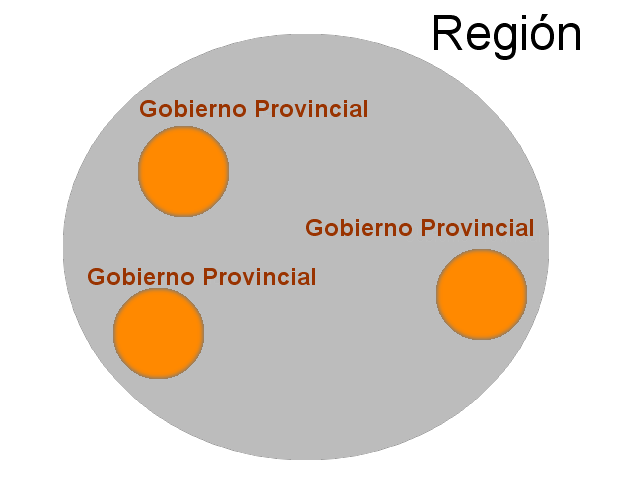
\includegraphics[scale=0.4]{regionProvincia.png}
\end{figure}

De �sta forma, se tiene un mejor control de los datos y los modelos de las diferentes provincias, adem�s de distribuir la ejecuci�n de una misma regi�n.

La comunicaci�n entre $Estaciones$ $Centrales$ pude realizarse por diferentes medios de comunicaci�n, ya sea por gsm o por Internet por ejemplo y eso estar� descripto en la descripci�n de funcionalidad del componente responsable de esa comunicaci�n. Esta comunicaci�n se realizar� mediante mensajes de control que permitan a una Estaci�n central, pedir resultados parciales de un modelo, o pedir informaci�n de ciertos sensores a otras Estaciones Centrales regionales.

\section{Estructura}

Para poder cumplir con estos requerimientos, como se dijo se deber�n agregar estaciones centrales de forma distribuida a lo largo de todo el pa�s.
Pero con la restricci�n de que exista a lo sumo una por provincia. Sumado a esto cada una de estas EC provinciales (ECP), tendr�n un sistema de
monitoreo (SMP) muy parecido al original, s�lo que tendr� las componentes fundamentales, las que son pertinentes al manejo provincial.

Esto no cambia, sin embargo, que exista una estaci�n central con todas las funcionalidades originales y tambi�n su sistema de monitoreo correspondiente.

Otro gran cambio que se realiza en cuanto a la forma de obtenci�n de datos de una TR es que la EC o ECP que necesite los datos de dicha TR tendr� que
suscribirse y estas cada vez que tengan un nuevo dato lo enviar�n a todos los suscriptos (publish/subscribe).
Este mecanismo tiene el limite del control provincial, las ECP s�lo se podr�n suscribir a las TR que est�n en la regi�n de la provincia. Si llegaran a necesitar
un dato de una TR en la misma regi�n pero en otra provincia, deber�n suscribirse a los datos de dicha TR a trav�s de la ECP que los controle.

El mecanismo de suscripci�n y publicaci�n de datos en una TR y en una EC o ECP ser�n polim�rficos, logrando de esta forma transparencia a la hora de notificar
y/o suscribirse a los datos.

Otro detalle importante en cuanto a la suscripci�n de estos datos, se podr�n hacer pidiendo un subconjunto de los sensores que posea la TR correspondiente.
Esta a su vez sabr� responder que tipo de sensores tiene presentes.

El �ltimo cambio que se realiza es que no s�lo se podr� una ECP suscribir a otra para pedir datos de alguna TR en su provincia con ciertos sensores, si no 
que tambi�n se podr� suscribir a datos parcial o totalmente calculados por un modelo en la EC o ECP.

\section{Nuevos componentes en la arquitectura}

Veamos ahora los nuevos componentes agregados a la arquitectura, cabe destacar para esta secci�n que s�lo se agregaron componentes en las TRs y las ECPs, 
los referentes al publish suscribe tanto de datos directos desde TRs a ECs como tambi�n los de datos crudos y resultados parciales y finales desde ECP a ECP.


Si bien no se agregaron nuevas componentes al sistema de monitoreo, se quitaron algunas, como por ejemplo los web services a la p�gina de la infraestructura en los SMP, los de las otras empresas podr�an estar o no de acuerdo a los criterios de la provincia, y lo mismo con el sistema e�lico, por eso preferimos mostrar en las im�genes posteriores el sistema de monitoreo de la primera entrega sin la parte web a la p�gina de infraestructura ya que la forma depende propiamente de cada una de las provincias.
\subsection{TR}

\begin{itemize}

\item \textbf{Publicador:} Este es el componente que se encargara de recibir las suscripciones que se env�an a la Comunicaci�n EC, guardando estos datos en 
la base de datos de la TR. Luego cuando el Sincronizador publique los datos a la Comunicaci�n EC, este �ltimo le pedir� todos suscriptos al Publicador y 
le enviar� los datos correspondientes.

\end{itemize}

\begin{figure}[H]
    \centering
    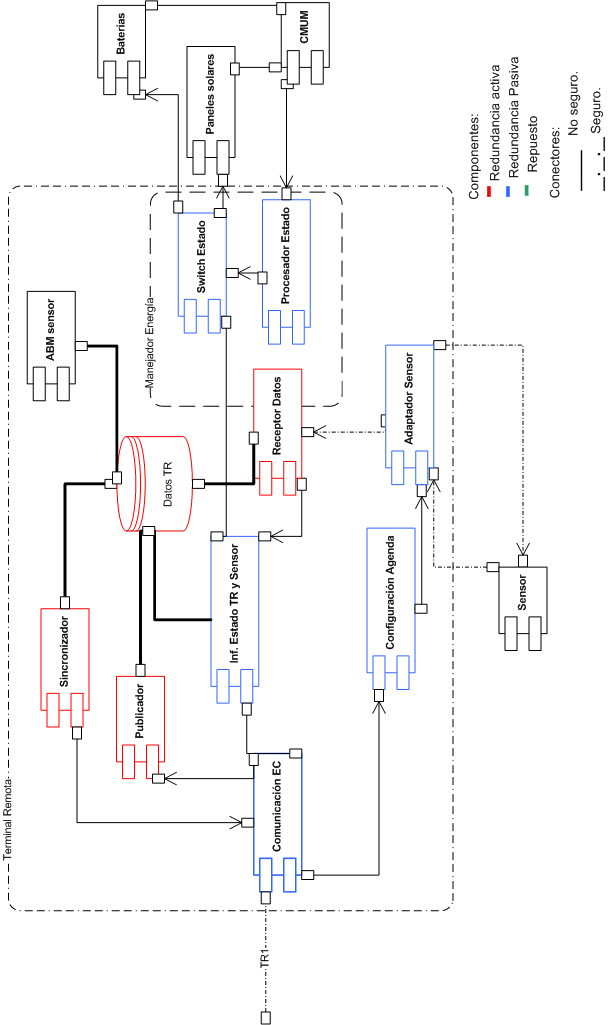
\includegraphics[scale = 0.6]{TR.png}
\end{figure}

\subsection{ECP}

Tenemos en esta parte grupos de componentes nuevos, unos encargados de la publicaci�n de datos que recibe directo de la TR hacia otra EC y un 
segundo grupo que se encarga de publicar y recibir los datos parciales y finales de los modelos entre ECs

\subsubsection{Datos Crudos}

\begin{itemize}

\item \textbf{Publicador TR:} Componente encargado de administrar las ECs suscriptas para obtener los datos crudos de las TRs administradas
por la EC. Se comunica con este componente la Recepci�n Segura, la cual le env�a los suscriptos y luego los pide cuando hay datos completos.

\item \textbf{Suscriptos TR:} Base en donde se guardan los datos de suscripciones para obtener la informaci�n cuando sea necesario.

\end{itemize}

\subsubsection{Resultados de Modelos}

\begin{itemize}

\item \textbf{Publicador Modelos:} Al igual que el componente Publicador TR este se encarga de administrar la informaci�n de las ECs suscriptas
tanto a resultados parciales de modelos como a resultados finales de los mismos.

\item \textbf{Suscriptos Modelos:} Base en donde se guardan los datos de suscripciones que administra el Publicador Modelos

\item \textbf{Intercambio Resultado:} Componente encargado de recibir un resultado parcial o total (enviado por el Procesador) para publicarlo 
a todos los suscriptos. Por medio del Publicador Modelos se entera cuales son estos suscriptos.
Cambien esta encargado de obtener los datos de otras ECs a las cuales se suscribe y luego guardarlo en Resultados otras ECs para que el Procesador los use
como resultados parciales o finales de los modelos de otras ECs

\item \textbf{Resultados otras ECs:} Base en donde se guardan los resultados parciales o totales obtenidos por suscripciones a modelos de otras ECs. 
Es el procesador el que levanta y utiliza estos datos.

\end{itemize}

\begin{figure}[H]
    \centering
    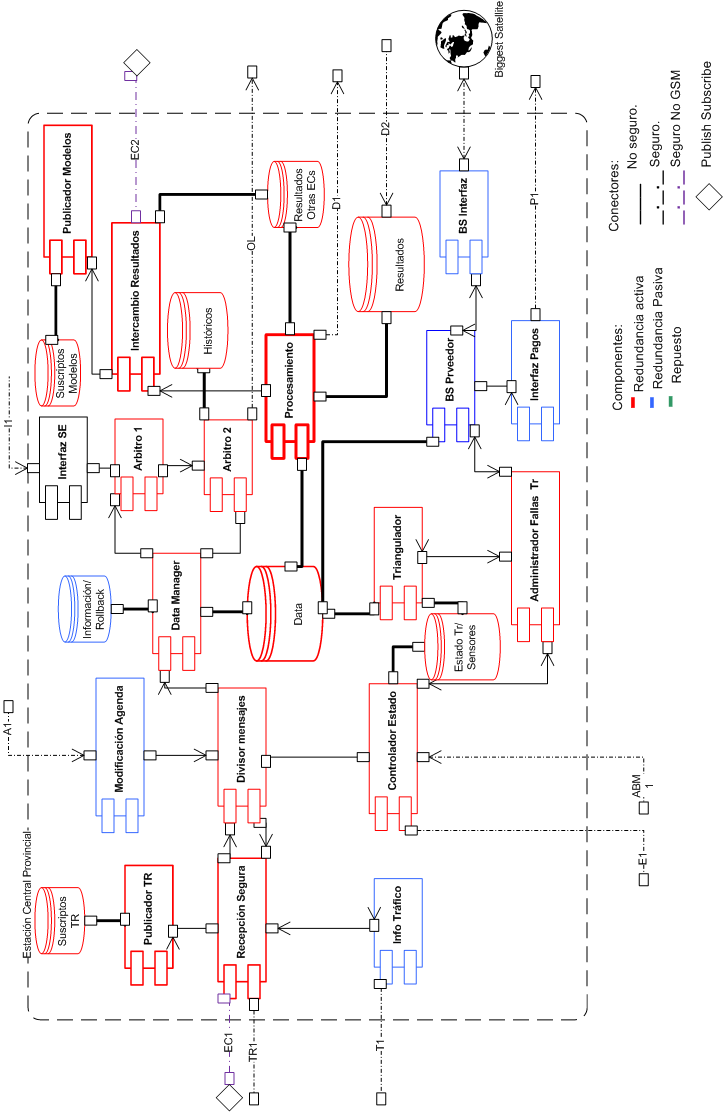
\includegraphics[scale = 0.6]{ECP.png}
\end{figure}

\subsection{SMP}

\begin{figure}[H]
    \centering
    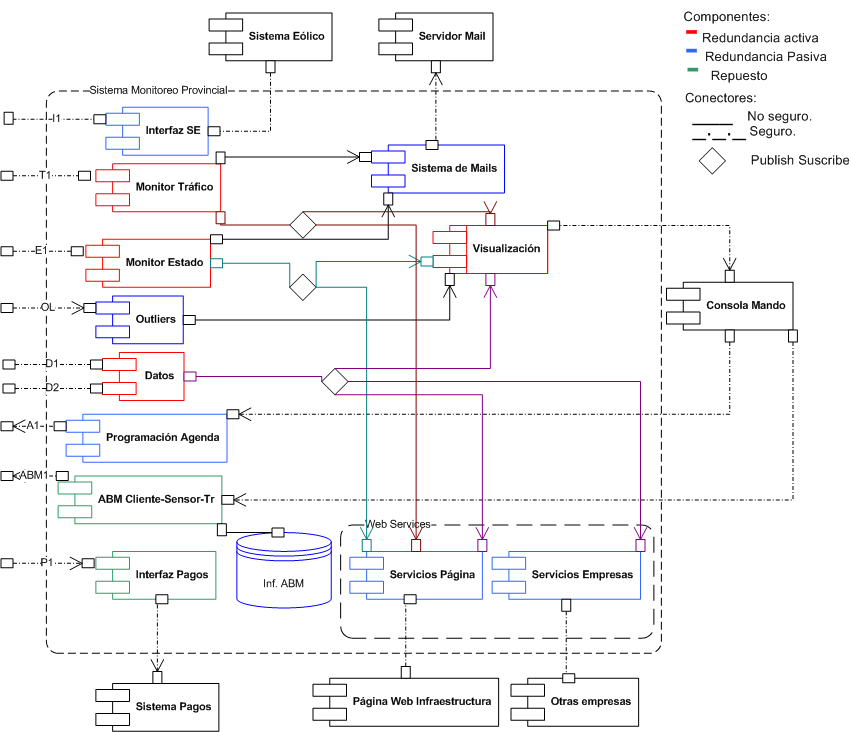
\includegraphics[scale = 0.6]{SMP.png}
\end{figure}


\clearpage

\newpage
\chapter{Impediment List}

En este capitulo se mostrar� la lista $Impediment$ $List$ con los problemas que pueden surgir en el proyecto y que afecte a su productividad y calidad. Estos estar�n agrupados por los $User$ $Story$ que se realizar�n en la primera iteraci�n.

\begin{enumerate}
\item US03: Trabajar en colaboraci�n con otras regiones (modelos)

\begin{itemize}
\item Algun problema realizando el protocolo de comunicaci�n.
\item Posibilidad de realizar mas cambios que lo planeado en la arquitectura para posibilitar la comunicaci�n y el intercambio de informacion.
\item Posibles problemas en la implementaci�n por uso de lenguajes o tecnicas desconocidas.
\item Aumento en el costo del testeo de los nuevos componentes y detecci�n de posibles errores en la arquitectura.
\end{itemize}

\item US08: Suscrpci�n de modelos a Trs

\begin{itemize}
\item Problemas definiendo las interfaces y el metodo de suscripci�n de los modelos.
\item Posibilidad de realizar mas cambios que lo planeado en la arquitectura.
\item Posibles problemas implementando la suscripci�n de estaciones centrales a trs.
\item Localizaci�n de errores en la arquitectura a la hora de realizar los testeos.
\item Problemas para definir correctamente la partici�n de las reglas.
\item Problemas realizando la unificaci�n de las particiones.
\item Posibles problemas para solucionar el problema de la colaboraci�n distribuida entro los modelos.
\item Complicaciones realizando el diagrama de objetos relacionado con la ejecuci�n de los modelos matematicos.
\end{itemize}

\item US10: Configuraci�n sencilla de colaboraci�n entre modelos

\begin{itemize}
\item Problemas para resolver la configuraci�n que permita la colaboraci�n entre modelos.
\item Localizaci�n de errores en la arquitectura a la hora de realizar los testeos.
\end{itemize}


\item US11: Varios algoritmos de evaluaci�n de reglas

\begin{itemize}
\item Posibles complicaciones realizando el diagrama de objetos para los algoritmos de evaluaci�n de reglas.
\end{itemize}

\end{enumerate}

\clearpage

\newpage
\chapter{Dise�o}


\section{Ideas llevadas a cabo}

En �ste cap�tulo se llevar� a cabo el dise�o especificado para los User Stories asociados al sprint tales que, si bien no necesitaban ser implementados, requer�an de un dise�o.

Estos user stories son aquellos referidos a la evaluaci�n de modelos utilizando diferentes algoritmos, de manera distribuida y a la f�cil configuraci�n entre las subpartes de un determinado modelo.

Para ello lo que se intent� llevar a cabo es la posibilidad de procesar un determinado modelo, siguiendo las reglas de descomposici�n asociadas a un determinado algoritmo. 

En la imagen que se puede ver a continuaci�n se refleja lo pensado por el grupo para lidiar con el requerimiento solicitado apra �sta parte del trabajo pr�ctico.

Comencemos a describir entonces �sta idea.

Existir�n, a diferencia del trabajo pr�ctico anterior algunas fuentes de datos m�s, no s�lo los datos sensados desde las terminales remotas asignadas a la ECP sino los provenientes de otras ECP relevantes. Todos estos datos de manera combinada
van a ser datos ''crudos" a procesar. Por otro lado vamos a tener tambi�n resultados parciales o totales provenientes de otras ECP los cuales ser�n utilizados en el procesamiento. Hasta aqu� todo lo referido al imput de procesamiento.

Por otro lado tendremos un modelo, un conjunto de reglas a aplicar para los datos, siguiendo la l�nea del trabajo pr�ctico anterior, la idea es que �stas reglas se refieran a variables o par�metros de alg�n tipo de almacenamiento de los datos, como pueden ser paquetes, diccionarios, etc, con la idea de no intervenir en la propia regla pasandole los datos que propiamente necesita.


La idea es que el tipo de procesamiento va a depender pr�cticamente del algoritmo encargado de procesarlo. Es decir, dado un determinado modelo y un conjunto de datos, el algoritmo ser� capaz de dividir las reglas en subpartes a su criterio, e intentar� correrlas en tantos procesadores como le convenga para agilizar el procesamiento. Por otro lado, una vez obtenidos los resultados, acturar� acordemente a lo que se solicite(Ej, pasarlo a otra componente, almacenarlo en una BD, etc).

Como se ver� en la descripci�n detallada del dise�o, itentaremos que el intercambio entre algoritmos se haga de manera sencilla y que adem�s la ejecuci�n concurrente, se pueda llevar a cabo de forma transparente al algoritmo. Con �sto �ltimo no contradecimos la idea de es el algoritmo quien determina las subpartes y c�mo se ejecutar�n, sino que intentaremos utilizar alguna clase adicional que se encargue de brindar fuentes de procesamiento cuando se lo requiera.

\begin{figure}[h]
\centering
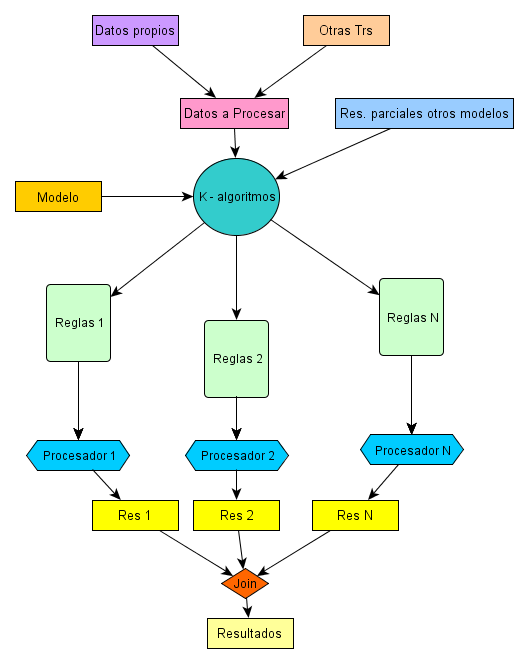
\includegraphics[scale=0.5]{../Disenio.png}
\end{figure}

\clearpage
\newpage


\section{Diagrama de clases}

En �sta secci�n describiremos como llevamos a un diagrama de clases las ideas mencionadas con anterioridad de modo tal de lograr una buena trazabilidad entre lo que pensamos y lo que vamos a llevar a cabo.


El diagrama correspondiente a dicha secci�n se puede observar al final de la misma. Cabe destacar que se utiliz� para las funciones una notaci�n similar a lenguages tipo C, C++, .Net o Java pero que su equivalente a Smalltalk o similires se puede realizar de manera sencilla, s�lo que la herramienta que utilizamos no lo permit�a. 


Pasemos entonces a enumerar las diferentes clases y las funcionalidades asociadas:

\begin{enumerate}

\item \textbf{Ejecutador Modelos: }Esta clase se va a encargar del manejo del procesamiento de los datos. Invocar� a otras clases para llevar a cabo cada uno de los pasos. 
	\begin{itemize}
  \item \textbf{ejecutarModelo: }Esta funci�n es la que en un determinado momento se utiliza para ejecutar un modelo. Cabe destacar que seguimos con la trazabilidad del trabajo pr�ctico anterior en cuanto que al pasarse el modelo a procesar, el mismo puede intercambiarse por otro, ademas se le pasa 3 par�metros m�s correspondientes a armadores y bases de datos, que ser�n comentadas a continuaci�n. 
  \end{itemize}

\item \textbf{BDP Access: }Esta clase se encarga de la comunicaci�n con la base de datos, de los datos a procesar en un determinado momento, ya sea los datos propios o los de otras Tr's.
	\begin{itemize}
  \item \textbf{datos : }Esta funci�n o mensaje retorna dado un tiempo los datos asociados correspondientes.
  \end{itemize}

\item \textbf{BDRP Access: }Esta clase se encarga de la comunicaci�n con la base de datos de los resultados parciales almacenados hasta el momento proveniente de otras ECP.
	\begin{itemize}
  \item \textbf{datos: }Dado un tiempo devuelve los datos correspondientes.
  \end{itemize}

\item \textbf{Armador Paquete: }Esta clase arma de alguna forma, una estructura o paquete con todos los datos necesarios para el procesamiento.
	\begin{itemize}
  \item \textbf{armar: }Dados datos a procesar y resultados parciales, arma una estructura correspondiente para procesar, en principio podr�a ser un diccionario.
  \end{itemize}

\item \textbf{Conjunto Reglas: }Esta clase si bien no era necesaria modelarla, muchas veces en Ingenier�a I nos solicitaban que aparezca para poder mostrar ciertas caracter�sticas deseables.
	\begin{itemize}
  \item \textbf{Iterador: }Como toda estructura de almacenamiento, puede proveer un iterador para recorrerla.
  \end{itemize}
  
\item \textbf{Regla: }Esta clase se corresponde con una determinada regla.
	\begin{itemize}
  \item \textbf{Ejecutar : }La idea es que dado un paquete de datos, la regla se ejecute, utilizando los datos de dicho paquete.
  \end{itemize}

\item \textbf{Estrategia: }Esta clase o bien es abstracta o bien es una interfaz, la idea es que un Ejecutador de modelos tenga una estrategia o algoritmo asociado para procesar el modelo. Este patr�n(Estrategy), es el que permite f�cilmente intercambiar el algoritmo de evaluaci�n de reglas.
	\begin{itemize}
  \item \textbf{aplicar: }Dados un conjunto de reglas y un paquete de datos tratar� de ejecutar las reglas utilizando esos datos.
  \end{itemize}
  
\item \textbf{Algoritmo 1: }Esta clase implementa una estrategia, la idea es que implemente la funci�n aplicar de la manera que le convenga.
	\begin{itemize}
  \item \textbf{join: }En este caso utiliza una funcion join para juntar los resultados de procesamientos intermedios, podr�a utilizar otra funci�n de acuerdo al algoritmo.
  \item \textbf{hacerAlgoUtil : }Corresponde a posibles funciones adicionales que implemente.
  \end{itemize}
    
\item \textbf{Fabrica Calculadores: } Se trata del patr�n Factory, la idea es fabricar calculadores cuando el algoritmo lo solicite para procesar un subconjunto de reglas. El calculador en principio podr�a ejecutarse en otro procesador, o bien ser un proceso independiente en un procesador.
	\begin{itemize}
  \item \textbf{calculador: }Devuelve un calculador.
  \item \textbf{stop: }Destruye una instancia de calculador cuando ya no es requerida.
  \end{itemize}
  
\item \textbf{Calculador: }Esta clase representa a los calculadores encargados de ejecutar las reglas.
	\begin{itemize}
  \item \textbf{calcular : }Dados datos y un conjunto de reglas las ejecutar�.
  \end{itemize}
\end{enumerate}


\begin{figure}[h]
\centering
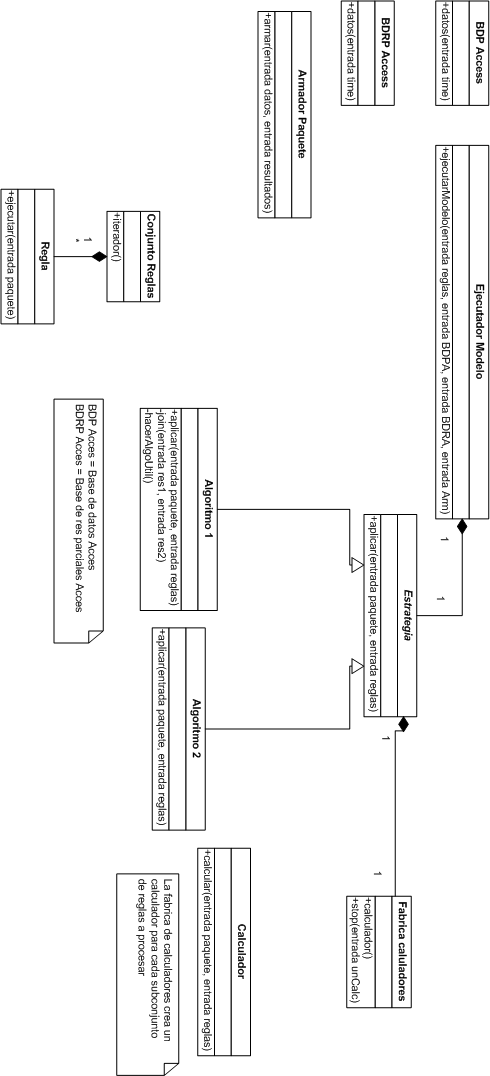
\includegraphics[scale=0.7]{../Disenio(2).png}
\end{figure}

\clearpage
\newpage


\section{Diagrama de objetos y secuencias}

Para �sta secci�n llevaremos a cabo una instancia del problema a modo de mostrar el funcionamiento esperado descripto anteriormente. 

Para ello realicezaremos un diagrama de objetos y un escenario correspondiente al mismo respresentado por varios diagramas de secuencias.

La idea es simple vamos a tener instancias de los principales clases que intervienen en el procesamiento y surgir�n algunos objetos m�s, propios de los escenarios elegidos.

Nuevamente los diagramas correspondientes se pueden observar al final de �sta secci�n para poder ir observando los mismos a medida que se lee el informe.

Comencemos con los objetos, vamos a tener instancias de los accesos a la base de datos, del ejecutor, del armador, del algoritmo, de las reglas y de la f�brica. Como resultado del escenario se podr�n notar la aparicion de intancias de calculadores, y subconjuntos de reglas con reglas asociadas. Esto es para que se pueda apreciar mejor el diagrama de secuencias.

Sigamos entonces explicando un poco el funcionamiento de los diagramas de secuencias elegidos. Vamos a contar b�sicamente el procedimiento ya que la comunicaci�n propiamente dicha es f�cilmente observable en los diagramas. La idea es que el eljecutor de modelos tomar� un modelo(conjunto de reglas), las bases de datos , y el armador. A su vez como se mencion� anteriormente el ejecutor tiene una estrategia asociada, en este caso el algoritmo 1. Entonces el ejecutor solicitar� los datos correspondientes a los accesos a las bases de datos para un determinado tiempo. Una vez hecho �sto solicitar� al armador que le provea un paquete con todos los datos necesarios para el procesamiento.

Cuando los datos ya est�n homogeineizados se delega la tarea de ejecuci�n al algoritmo o estrategia. El algoritmo va a dividir las reglas en subpartes de acuerdo a su conveniencia o su manera de operar, en este caso en 2 partes, y para ejecutar concurrentemente estas partes solicitar� a la fabrica dos calculadores. A cada uno de los calculadores le solicitar� que ejecute el correspondiente subconjunto de reglas, y una vez obtenidos los datos, los unificar� para devolver un resultado final.

Es importante destacar que cuando un calculador finalice su ejecuci�n, el algoritmo le solicitar� a la fabrica que elimine o detenga el funcionamiento de dicho calculador ya que no es m�s necesario. La f�brica destruir� �ste calculador, y liberar� su relaci�n con un determinado procesador para que pueda ser utilizado nuevamente cuando sea solicitado.

Finalmente el calculador ejecutar� cada una de las reglas solicitadas y luego devolver� el resultado de dicha ejecuci�n.


\begin{figure}[h]
\centering
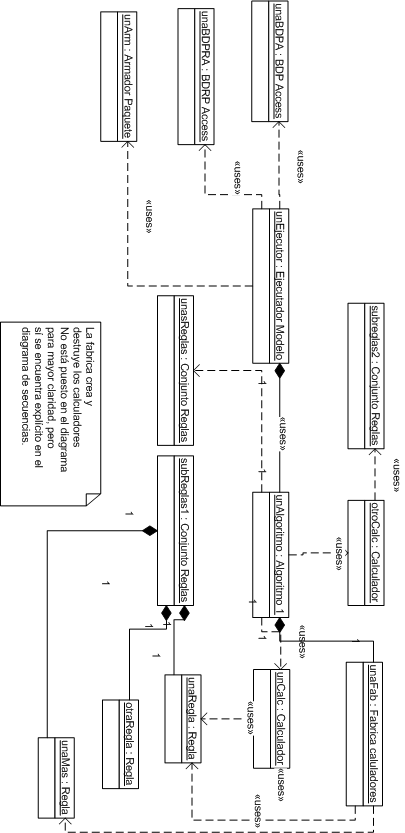
\includegraphics[scale=0.8]{../Disenio(3).png}
\end{figure}

\begin{figure}[h]
\centering
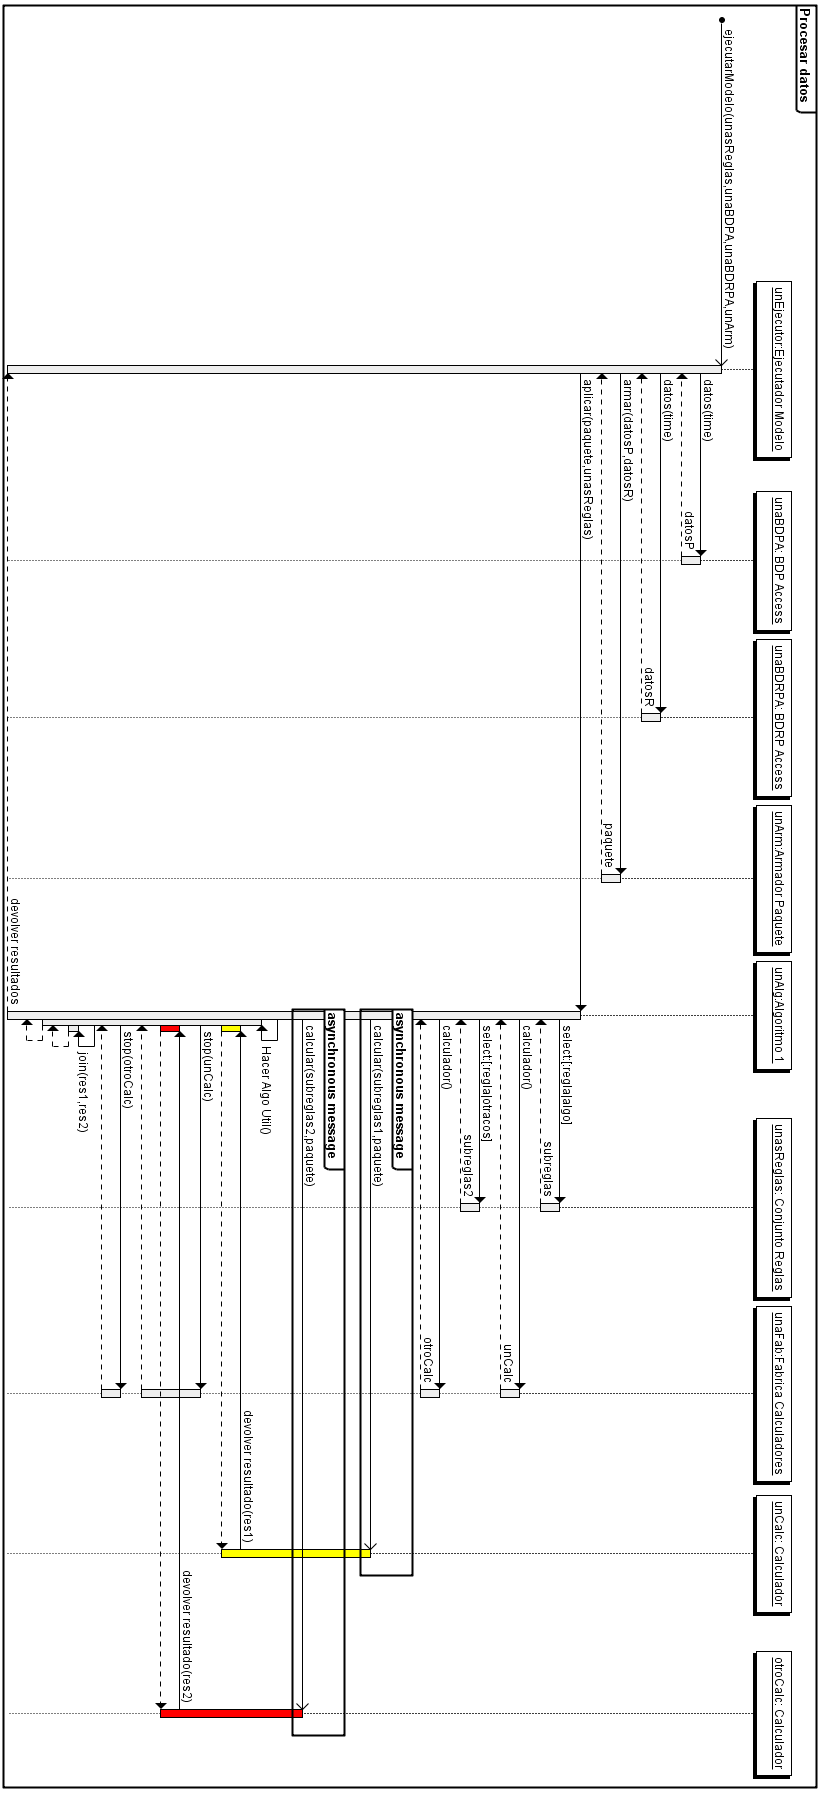
\includegraphics[scale=0.55]{../secuencias.png}
\end{figure}

\begin{figure}[h]
\centering
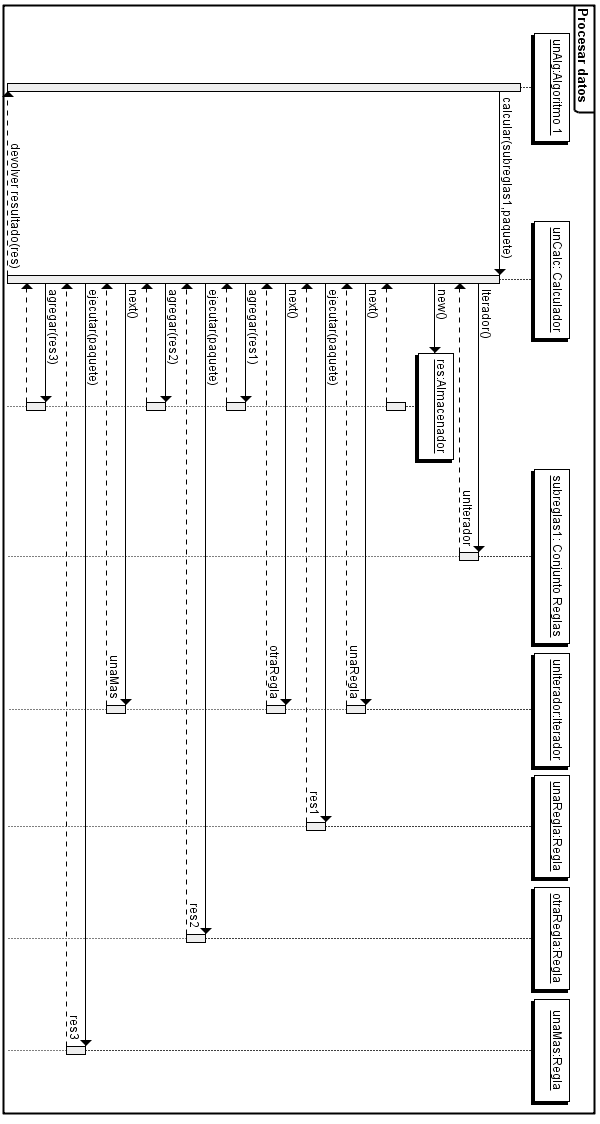
\includegraphics[scale=0.8]{../aplicarReglas.png}
\end{figure}

\begin{figure}[h]
\centering
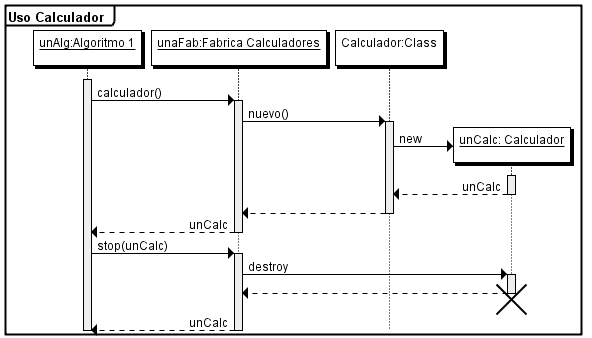
\includegraphics[scale=0.7]{../creaYDestruyeCalc.png}
\end{figure}

\clearpage
\newpage
\clearpage

\newpage
\chapter{Comparaci�n UP-Scrum}


\clearpage

\newpage
\chapter{Bibliograf�a}

\clearpage

\newpage
\chapter{Conclusi�n}

Si bien se sabe que el dise�o del proyecto est� en sus primeros pasos, con lo realizado en esta preentrega, se tiene una especificaci�n relativamente exhaustiva de las cosas mas importantes del dominio del problema. Con estos datos se pudo definir la base de la arquitectura del sistema, que si bien puede cambiar, se supone que no afectara gravemente el dise�o original, ni traer� problemas que posterguen demasiado el proyecto.

Para realizar esta afirmaci�n nos basamos en que al realizar el diagrama contextual (que sirve en este caso de arquitectura), tomamos en cuenta varios de los requerimientos y atributos de calidad planteados inicialmente, proponiendo una arquitectura que es incremental, en cuanto a que se pueden agregar Terminales Remotas, y en cuanto a que se puede incrementar el poder de c�mputo. Tambi�n es resistente a fallas en las transmisiones, ya que se implementara un protocolo confiable entre las TRs y la Estaci�n Central y tambi�n es resistente a fallas en los equipos, dado que se van a poder subsanar la ca�da de una TR triangulando o utilizando un servicio externo. Adem�s se contempla el hecho de tener comunicaci�n con diferente tipo de sistemas, ya sean clientes externos (como AgroTop), proveedores de servicio (Biggest Satelite) y usuarios internos, encargados de monitorear el estado del sistema.

Se dise�� un plan que tiene en cuenta tiempos de entrega y de desarrollo que son acotados, por esta raz�n se tuvo que identificar dependencias entre las funcionalidades principales que se detectaron, como as� su importancia y complejidad dentro del sistema.

Como se conoce estos m�todos llevan bastante tiempo, pero ayudan a tener un control del proyecto y tener luego un hilo de ejecuci�n bien definido que permitir� optimizar el desarrollo del sistema durante el tiempo. Teniendo en cuenta el contexto en el que se realiz� el trabajo creemos haber cumplido las expectativas en cuanto a los requerimientos pedidos para esta entrega.

\clearpage
\label{LastPage}
\end{document}
